% File: analyse.tex
% Date: Fri Aug 31 01:14:59 2012 +0800
% Author: Yuxin Wu <ppwwyyxxc@gmail.com>
\section{Results and Analysis}


\begin{enumerate}

\item 处理器核数不同时运行时间比较:

\begin{lstlisting}

$ ./pthread -n 2 -b 10000 -t 10                                                                                                                                                                                                                
36.127635 seconds in total...
$ ./pthread -n 4 -b 10000 -t 10                                                                                                                                                                                                                
18.336705 seconds in total...
$ ./pthread -n 6 -b 10000 -t 10                                                                                                                                                                                                                
12.532974 seconds in total...
$ ./pthread -n 8 -b 10000 -t 10                                                                                                                                                                                                                
9.650894 seconds in total...
$ ./pthread -n 10 -b 10000 -t 10
7.912135 seconds in total...
$ ./pthread -n 12 -b 10000 -t 10
6.736707 seconds in total...

$ mpirun -n 2 ./mpi -b 10000 -t 5
36.700927 seconds in total...
$ mpirun -n 4 ./mpi -b 10000 -t 5                                                                                                                                                                                                              
14.856551 seconds in total...
$ mpirun -n 8 ./mpi -b 10000 -t 5                                                                                                                                                                                                              
17.607959 seconds in total...
$ mpirun -n 12 ./mpi -b 10000 -t 5                                                                                                                                                                                                             
13.325384 seconds in total...
\end{lstlisting}
	由以上数据可以得出,pthread与MPI在核数与CPU数相等时效率较高,这与以往的经验吻合.

\item 各并行方式下程序运行时间比较:
\begin{lstlisting}
$ ./pthread -b 10000 -t 10
6.735550 seconds in total...
$ ./omp -b 10000 -t 10                                                                                                                                                                                                                         
20.149873 seconds in total...
$ mpirun -n 12 ./mpi -b 10000 -t 10
26.785754 seconds in total...
$ ./seq -b 10000 -t 10
70.296430 seconds in total...
\end{lstlisting}

本程序的并行效率比较结果表明,pthread效率最高,其次是OpenMP与MPI.这与上一个作业的结果吻合.

\item 球个数不同时运行时间比较:

	\begin{table}[h]
		\centering

		\begin{tabular}{c|c|c|c|c|c|c|c|c}
			\hline
			& 2000	    &5000       &10000      &15000	    &20000	    &30000      &40000			&50000\\\hline
			24  & 7.474266  &15.150455  &17.909214  &23.538911  &32.357338  &58.790446  &94.269225  & 138.547335 \\
			48  & 6.104528  &16.262802  &16.294989  &18.443990  &23.920497  &39.704812  &56.713508  & 79.303986  \\
			60  & 5.965712  &10.075106  &15.898907  &18.610584  &22.252957  &32.892880  &49.755771  & 68.303462  \\
			72  & 4.468587  &10.164223  &15.730339  &19.156377  &20.973644  &30.322637  &43.577078  & 60.674458  \\\hline

		\end{tabular}
		\caption{不同球数,处理器个数下运行时间统计(秒)}
	\end{table}

	\begin{figure}[H]
		\centering
		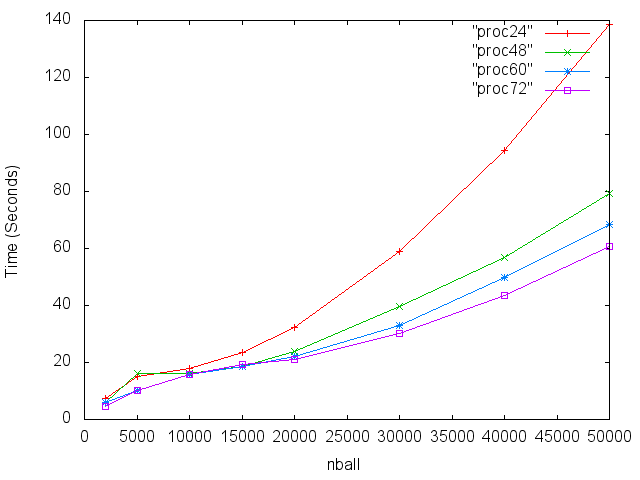
\includegraphics[scale=0.7]{res/ball.png}
	\end{figure}
	可以看出,当核数较少时,时间关于球数大约呈二次函数关系.这与算法$ O(n^2)$的复杂度相吻合.
	核数多时,由于数据量不够大,因此对于球少的情形,并没有显著的加速.


\item 	多核心大数据运行时间比较:

	\begin{figure}[H]
		\centering
		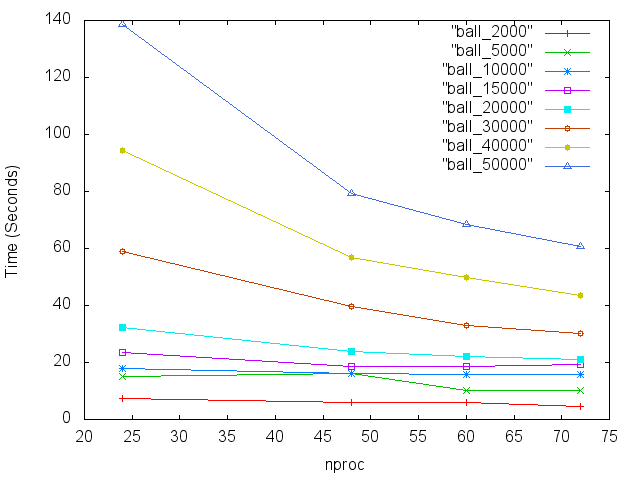
\includegraphics[scale=0.7]{res/proc.png}
	\end{figure}
	可以看出,数据量较小时,多线程的加速效果几乎不可见,这是由于在每个循环周期内,程序会调用两次\verb|NBody::share_data()|来共享计算出的数据,
	每次调用需要广播\verb|MAXN * 4|个\verb|double|,对通信负载非常大.
	但由于题目的特殊性,每次计算都要求获取其余所有物体上一循环结束时的信息,因此这种通信是必不可少的,
	当数据量增大时,多线程的加速效果开始变得明显.

\item 循环次数不同时运行时间比较:
	\begin{figure}[H]
		\centering
		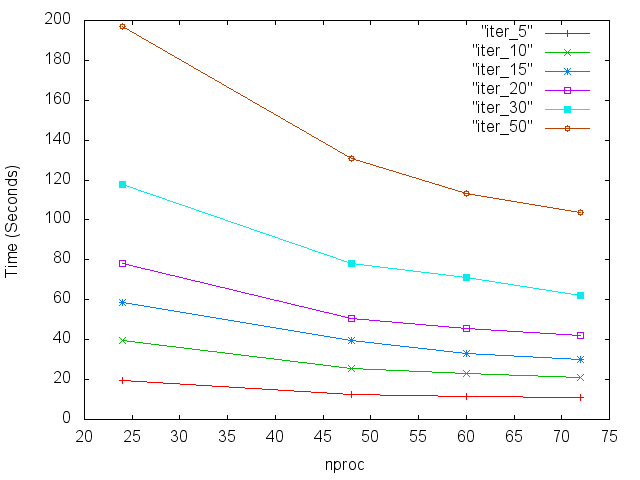
\includegraphics[scale=0.7]{res/iter.png}
	\end{figure}

	从上图中可以看出,循环次数与时间大约成正比.同时还可以发现,循环次数较多时,加速比变得不明显.
	这同样是因为,每次循环结束时,MPI各进程间需要广播数据.

\item 程序效能分析:

	使用gprof,对程序(以pthread版本为例)效能分析部分结果如下:

\begin{lstlisting}[basicstyle=\scriptsize\ttfamily]
$ gprof ./pthread gmon.out 
Flat profile:

Each sample counts as 0.01 seconds.
time   seconds   seconds  calls     name    
40.01     0.34     0.34  4871892    Body::cal_vel(Body const&, double)
31.78     0.61     0.27  4088280    col_time(Body const&, Body const&, double)
9.41      0.69     0.08  5809513    overlap(Body const&, Body const&)
7.06      0.75     0.06  5657909    operator*(double, Vec const&)
5.88      0.80     0.05    15036    NBody::collision_change(int)
3.53      0.83     0.03  4324526    tooclose(Body const&, Body const&)
\end{lstlisting}

	由以上结果,可以看出程序的大部分计算花费在计算引力(\verb|cal_vel()|)与碰撞(\verb|col_time()|,\verb|collision_change()|)上,
	这两个部分包含大量浮点运算. 上表中的\verb|overlap()|与\verb|tooclose()|函数是用于判断物体之间的一些相对位置关系的,
	使用它们使得我的程序展示效果更好,可以看出明显的引力与碰撞效果,没有太多的异常运动,但其中包含的浮点运算(见\secref{theory})消耗了不少资源.
\end{enumerate}
